\section{Approach}
\label{Sec:Approach}

	Our DOM based Code-completion approach consists of 3 phases. 1) DOM analysis, 2) Code analysis, and 3) Suggestion generation. The \emph{DOM analysis} phase (\figref{DOM-Analysis}) involves crawling the web application and generate list of \css selectors present within the DOM states. The \emph{Code analysis} phase (\figref{Code-Analysis}) involves analyzing the \javascript code, creating list of in-scope variables and intercepting the DOM API calls that include reading and writing to the DOM. The results from the above two phases are passed to the \emph{suggestion generation} phase (\figref{Suggestions}) and combined to generate list of auto-complete suggestions that are presented to the developer.
	
	\subsection{Usage Model}
	\label{Sec:Model}
		Because we focus on providing auto-complete for DOM based interactions, we assume that the developer has access to the web application under development. If the developer does not have access to the running web application, we assume that the developer has access to the HTML template of the website. Further, we assume that the JavaScript code within the editor is partially complete. By partially complete we refer to \javascript code that is syntactically correct and all the variables in use are defined and there are no global variables in use.
		
		Our approach is designed to provide code completion suggestions for \javascript-DOM interactions within the \javascript code. The input required from the developer is either of the function calls \texttt{querySelector}, \texttt{getElementById}, \texttt{getElementsByTagName}, or \texttt{getElementsByClassName} and name of the parent object calling these functions.
	
	
		The output of our approach is a list of tag names, id's or classes when the developer is trying to access any DOM element within the \javascript code. The generated list is dependent on 1) \javascript variables in scope 2) Scope of parent element within DOM 3) Additions / deletions made to the DOM within the available code paths.
	
	\subsection{DOM Analysis}
	\label{Sec:DOM-Analysis}
		\begin{figure}
		%	\begin{mdframed}
			\centering
			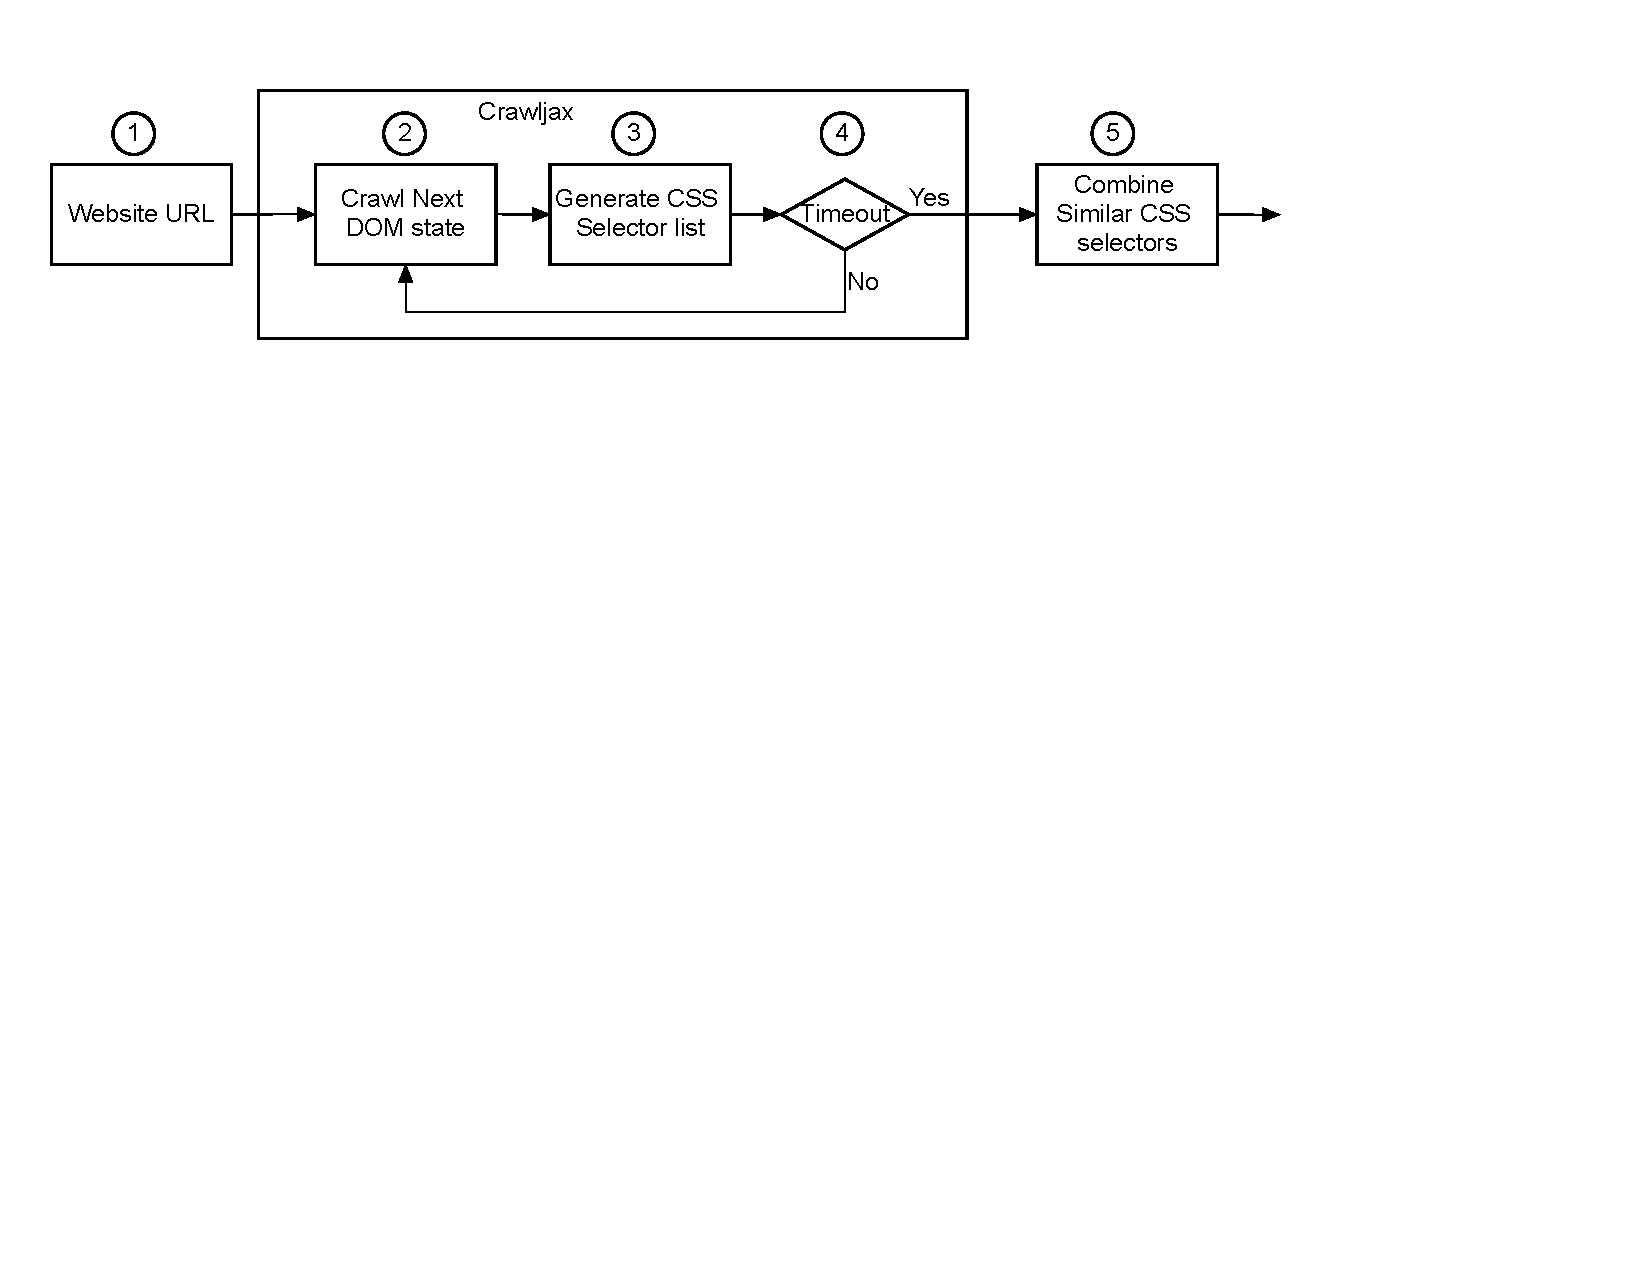
\includegraphics[width=85mm]{images/dom_analysis.pdf}
		%	\end{mdframed}
			\caption{DOM Analysis}
			\label{Fig:DOM-Analysis}
		\end{figure}
		In the DOM analysis phase, the corresponding web application is crawled (Step 2) using Crawljax \cite{crawljax:tweb12} to collect information about the DOM hierarchy. The information about DOM hierarchy is then stored in the form of \css selectors\footnote{\css selectors are the patterns used to select particular DOM element} (Step 3). Each leaf node in the DOM is expressed as a sequence of tag name, id's and classnames found in the hierarchy. As the number of DOM states within the website can be infinite, a timeout limit is set by the user. When one particular DOM state is stored in the form of \css selectors, the crawler moves to the next state. The process is continued until the timeout limit is reached (Step 4). Once the timeout has reached, the \css selectors generated from different DOM states are combined (Step 5) to generate a superset of \css selectors which are then used in the later phase.
		
		\headbf{Converting DOM to \css Representation}
		Every element within the DOM hierarchy can be addressed as a space separated sequence of nodes beginning from the root node. Each node is a DOM element and can be represented as a combination of tag name, id and list of classes attached to the element. For example for \figref{Example} the \texttt{li} elements can be represented as follows:
			
		\begin{quote}
			\texttt{div\#site-navigation ul.nav-menu.toggled-on li}
		\end{quote}
			
		To represent complete DOM tree in terms of \css selectors, we focus on all the leaf nodes within the tree, \ie the elements within DOM that does not have any child element. For every leaf node we generate a sequence of its \css selectors, therefore covering all the DOM elements present within the DOM tree. The list of \css selectors for each DOM state are then accumulated together to generate a superset of \css selector strings. The \css representation of the DOM tree for a single DOM state holds the following properties:
		\begin{itemize}
			 \item Each word represents a node in the DOM tree with a combination of tag name(required), class name(if present) and id(if present).
			 \item Each row starts with the root element and traverses to one of the leaf nodes i.e each row represents one path from root node to leaf nodes.
			\item Number of rows is equal to number of leaf nodes.
			 \item Number of words in each string represents the depth of particular path
		\end{itemize}
		
		As the number of crawled DOM states increases, the number of rows in the \css representation increases exponentially, therefore increasing the space and time complexity of the approach. To effectively provide code-completion suggestions within a decent time frame, we need to minimize the \css representation of the superset that is generated after the timeout is reached.
		
		\begin{description}
			\item[Removing duplicates from \css Representation]
			The two leaf nodes in the DOM tree that follow exactly similar DOM hierarchy \ie they have exactly same \css representation, we can remove one of them. For example in \figref{Example} the 2 \texttt{li} elements follows same DOM hierarchy therefore we can consider only one of them for the analysis.
		
			\item[Combining Similar IDs]
			Two rows within the \css based representation that follow the following criteria are the combined to form a single row. 

			\begin{itemize}
				\item The distance between the root node and the leaf node should be equal.
				\item Tag names should be exactly similar at each level of hierarchy.
				\item Classes attached to each tag should be exactly same.
			\end{itemize}

			For example:
			
			\begin{quote}
				\texttt{ul.nav-menu.toggled-on li\#item1}
	
				\texttt{ul.nav-menu.toggled-on li\#item2}
			\end{quote}

			In the above two sequences, distance between root node and leaf node for the both the sequences is 1, tag sequence for the sequences is \texttt{ul li}. Classes attached to each element are exactly same. To replace the above two sequences, we generate a new sequence that has exactly same length, tag sequence and classes attached to those tags. We then combine ids that differ in the original sequences and add all of these in the new sequence. The new sequence generated looks like the following sequence:

			\begin{quote}
				\texttt{ul.nav-menu.toggled-on li\#item1\#item2}
			\end{quote}


			\item[Combining Similar Classes]
			Two rows within the \css based representation that follow the following criteria are the combined to form a single row. 
			
			\begin{itemize}
				\item The distance between the root node and the leaf node should be equal.
				\item Tag names should be exactly similar at each level of hierarchy.
				\item IDs attached to each tag should be exactly same.
			\end{itemize}

			For example:
			\begin{quote}
				\texttt{ul.nav-menu.toggled-on li.item1}
	
				\texttt{ul.nav-menu.toggled-on li.item2}
			\end{quote}

			In the above two sequences, distance between root node and leaf node for the both the sequences is 1, tag sequence for the sequences is \texttt{ul li}. Ids attached to each element are exactly same. With the approach similar to the previous case the new sequence is generated.

			\begin{quote}
				\texttt{ul.nav-menu.toggled-on li.item1.item2}
			\end{quote}
		
		\end{description}
	
	\subsection{Code Analysis}
	\label{Sec:Code-Analysis}
		\begin{figure}
		%	\begin{mdframed}
			\centering
			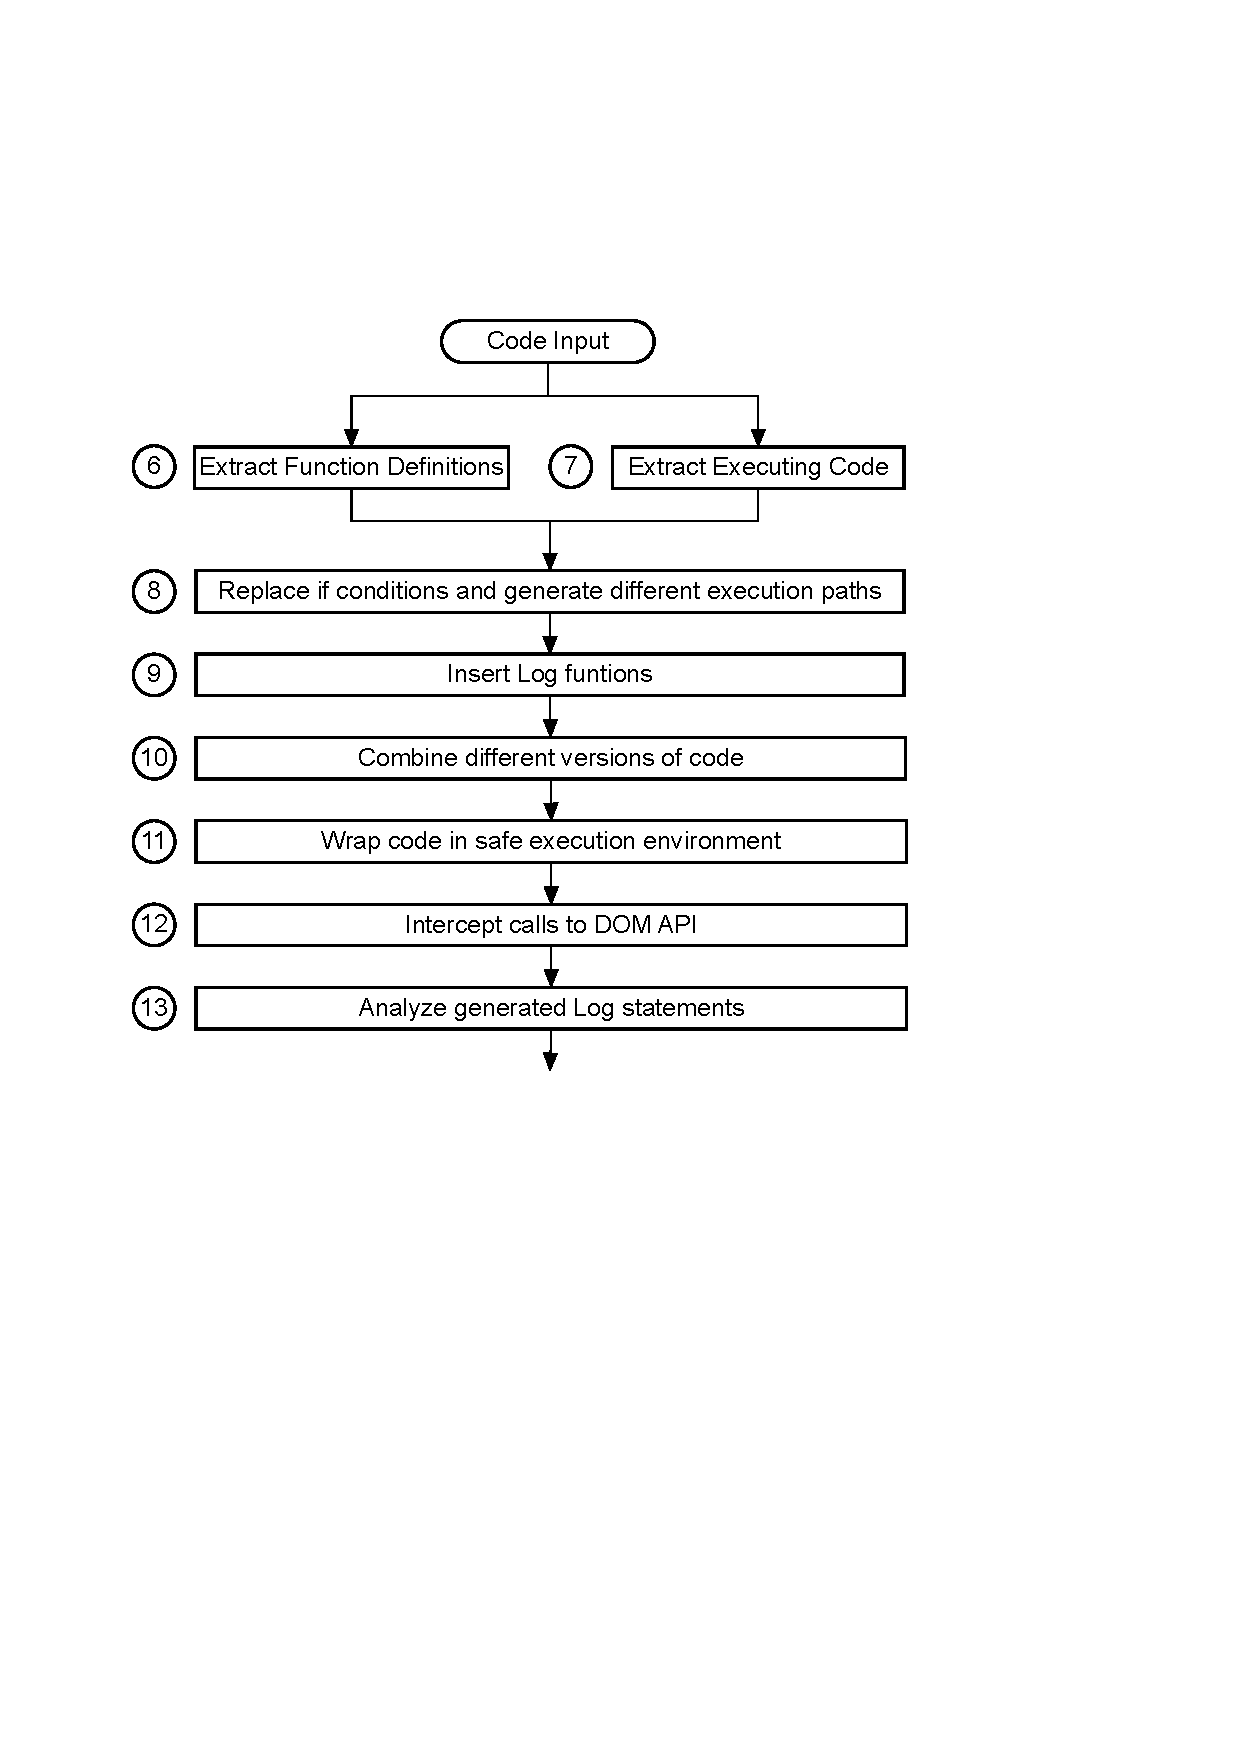
\includegraphics[width=85mm]{images/code_analysis.pdf}
		%	\end{mdframed}
			\caption{Code Analysis}
			\label{Fig:Code-Analysis}
		\end{figure}
	
	\subsection{Suggestion Generation}
	\label{Sec:Suggestions}
		\begin{figure}
		%	\begin{mdframed}
			\centering
			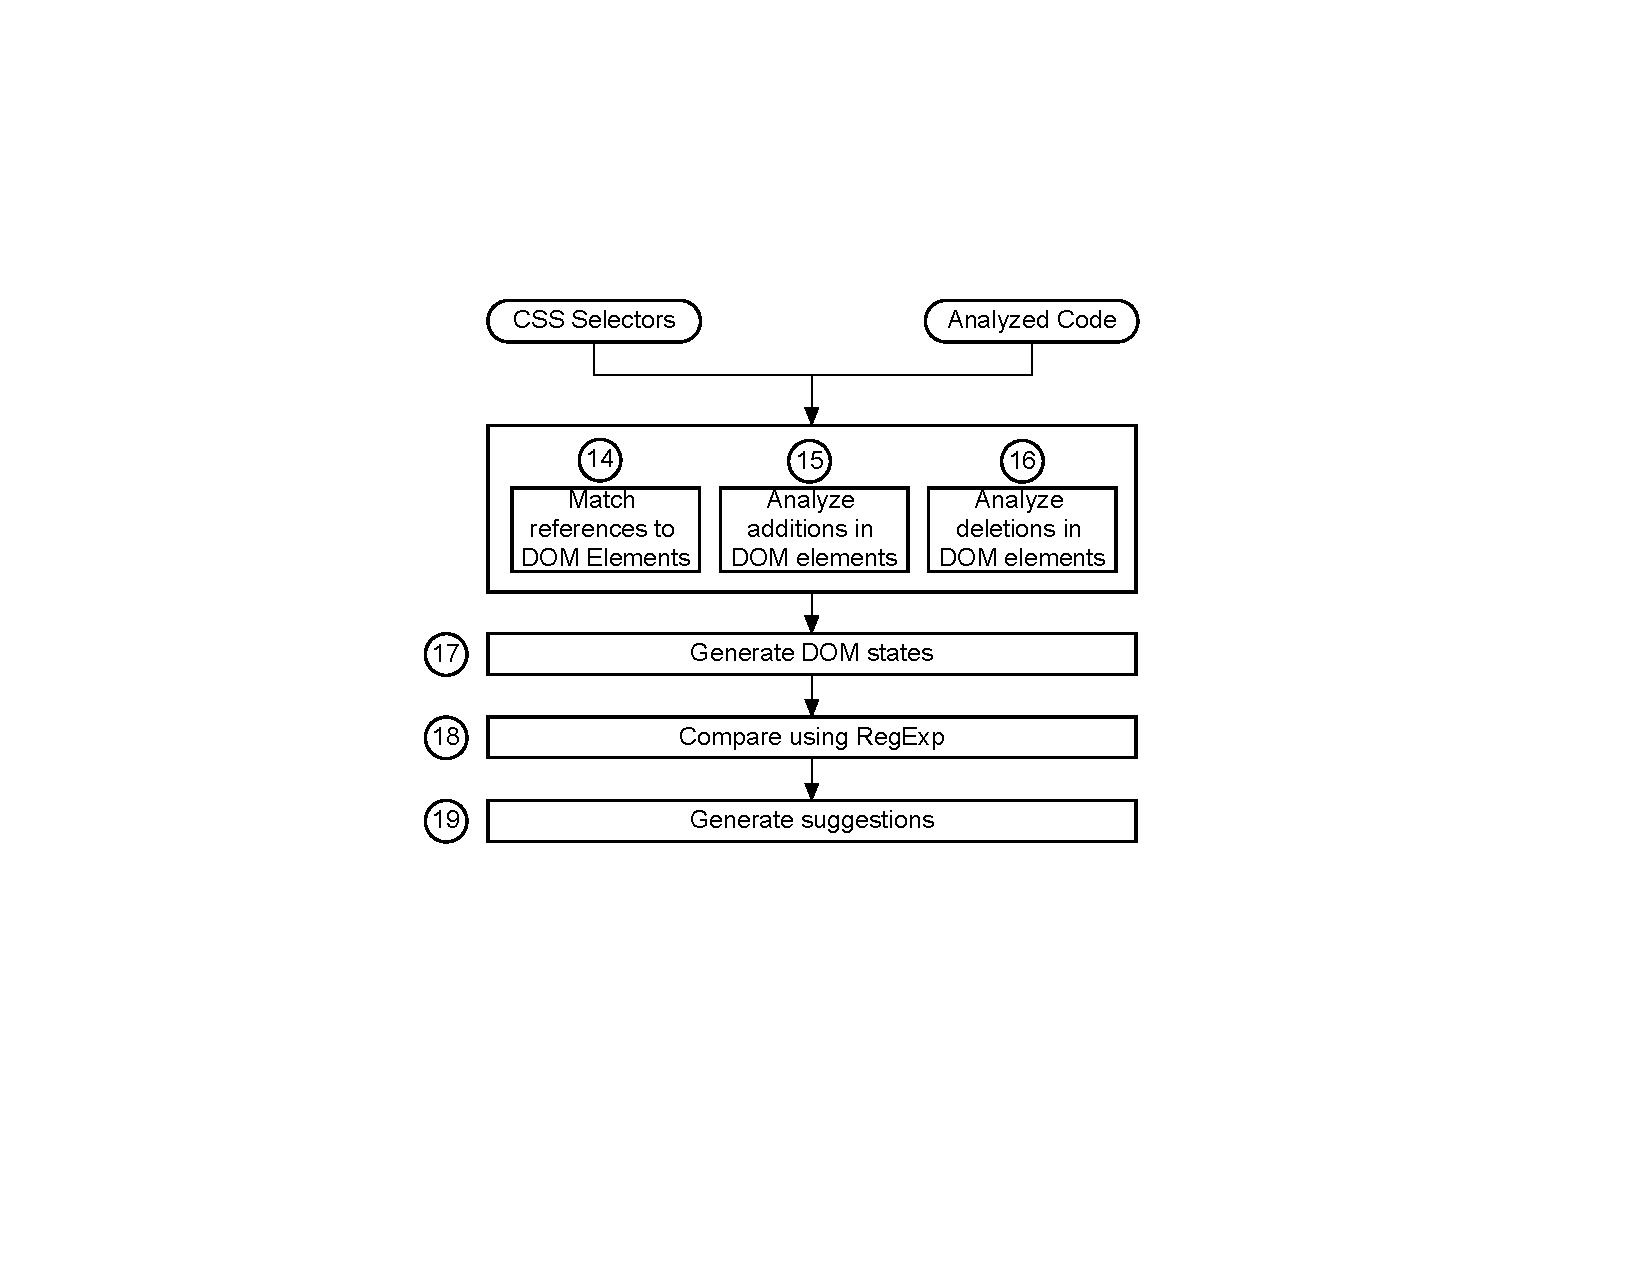
\includegraphics[width=85mm]{images/suggestions.pdf}
		%	\end{mdframed}
			\caption{Suggestion Generation}
			\label{Fig:Suggestions}
		\end{figure}